% SUPPLEMENTARY MATERIAL
% !Rnw weave = knitr
% -*-coding:latin-1-*-
\RequirePackage{fix-cm}

\documentclass[paper=a4,notitlepage,DIV=12]{scrartcl}\usepackage[]{graphicx}\usepackage[]{color}
%% maxwidth is the original width if it is less than linewidth
%% otherwise use linewidth (to make sure the graphics do not exceed the margin)
\makeatletter
\def\maxwidth{ %
  \ifdim\Gin@nat@width>\linewidth
    \linewidth
  \else
    \Gin@nat@width
  \fi
}
\makeatother

\definecolor{fgcolor}{rgb}{0.345, 0.345, 0.345}
\newcommand{\hlnum}[1]{\textcolor[rgb]{0.686,0.059,0.569}{#1}}%
\newcommand{\hlstr}[1]{\textcolor[rgb]{0.192,0.494,0.8}{#1}}%
\newcommand{\hlcom}[1]{\textcolor[rgb]{0.678,0.584,0.686}{\textit{#1}}}%
\newcommand{\hlopt}[1]{\textcolor[rgb]{0,0,0}{#1}}%
\newcommand{\hlstd}[1]{\textcolor[rgb]{0.345,0.345,0.345}{#1}}%
\newcommand{\hlkwa}[1]{\textcolor[rgb]{0.161,0.373,0.58}{\textbf{#1}}}%
\newcommand{\hlkwb}[1]{\textcolor[rgb]{0.69,0.353,0.396}{#1}}%
\newcommand{\hlkwc}[1]{\textcolor[rgb]{0.333,0.667,0.333}{#1}}%
\newcommand{\hlkwd}[1]{\textcolor[rgb]{0.737,0.353,0.396}{\textbf{#1}}}%

\usepackage{framed}
\makeatletter
\newenvironment{kframe}{%
 \def\at@end@of@kframe{}%
 \ifinner\ifhmode%
  \def\at@end@of@kframe{\end{minipage}}%
  \begin{minipage}{\columnwidth}%
 \fi\fi%
 \def\FrameCommand##1{\hskip\@totalleftmargin \hskip-\fboxsep
 \colorbox{shadecolor}{##1}\hskip-\fboxsep
     % There is no \\@totalrightmargin, so:
     \hskip-\linewidth \hskip-\@totalleftmargin \hskip\columnwidth}%
 \MakeFramed {\advance\hsize-\width
   \@totalleftmargin\z@ \linewidth\hsize
   \@setminipage}}%
 {\par\unskip\endMakeFramed%
 \at@end@of@kframe}
\makeatother

\definecolor{shadecolor}{rgb}{.97, .97, .97}
\definecolor{messagecolor}{rgb}{0, 0, 0}
\definecolor{warningcolor}{rgb}{1, 0, 1}
\definecolor{errorcolor}{rgb}{1, 0, 0}
\newenvironment{knitrout}{}{} % an empty environment to be redefined in TeX

\usepackage{alltt}
\pdfminorversion=4 % needed to ensure PDF version 1.4 for Journal tools
\usepackage{siunitx}
\usepackage{fixltx2e}
\usepackage{setspace}
\usepackage{array}
\newcolumntype{L}[1]{>{\raggedright\let\newline\\\arraybackslash\hspace{0pt}}m{#1}}
\usepackage{lineno}
\usepackage{amsmath}
\usepackage{amsfonts}
%\usepackage{amsthm}
\usepackage{graphicx}
\usepackage{latexsym}
\usepackage[numbers,sort&compress]{natbib}
\citestyle{nature}
\usepackage{nomencl}
%\usepackage{svninfo}
\usepackage[latin1]{inputenc}
\usepackage[T1]{fontenc}
\usepackage{lmodern}
\usepackage[activate={true,nocompatibility},final,tracking=true,kerning=true,spacing=true,factor=1100,stretch=10,shrink=10]{microtype}
\usepackage{textcomp}
\usepackage{eurosym}
\usepackage{upgreek}
\usepackage{setspace}
\usepackage{gensymb}
\usepackage[colorinlistoftodos,disable]{todonotes} % disable 
\usepackage{hyperref}
\newcommand{\g}[1]{\emph{#1}}

\makenomenclature
\let\nc\nomenclature

\newcommand{\piqe}{\left(\pi_0 \ Q \ e^{tQ}\right)_i}
\newcommand{\piqqe}{\left(\pi_0 \ Q^2 \ e^{tQ}\right)_i}
\newcommand{\pie}{\left(\pi_0 \ e^{tQ}\right)_i}

\newcommand{\field}[1]{\mathbb{#1}}
\newcommand{\C}{\field{C}}
\newcommand{\R}{\field{R}}
\newcommand{\N}{\field{N}}
\newcommand{\Q}{\field{Q}}
\newcommand{\A}{\ifmmode{\field{A}}      \else{$\field{A}$}\fi}
\renewcommand{\P}{\field{P}}

\DeclareMathOperator*{\argmax}{argmax}
\DeclareMathOperator*{\Var}{Var}
\DeclareMathOperator*{\modell}{Modell}
\DeclareMathOperator*{\rang}{rang}
\DeclareMathOperator*{\Mn}{\ifmmode{{\bf M(n;\R) }}\else{$\bf M(n;\R)  $}\fi}
\DeclareMathOperator*{\cof}{cof}
\DeclareMathOperator*{\adj}{Adj}
\DeclareMathOperator*{\tr}{tr}
\DeclareMathOperator*{\EMP}{{\boldmath EMP}}
\graphicspath{{../figures/}}

%% florian added:
%\usepackage[usenames,dvipsnames]{xcolor}
\usepackage{color}
%\newcommand{\todo}[1]{\textbf{\color{red} #1}}
\newcommand{\fm}[1]{{\color{BlueGreen} #1}}
\newcommand{\revised}[1]{{\color{blue} #1}}
\definecolor{gray}{rgb}{0.6,0.6,0.6}
\newcommand{\texttext}{\emph{\color{gray}`Twas brillig, and the slithy
toves/ Did gyre and gimble in the wabe:/ All mimsy were the
borogoves,/ And the mome raths outgrabe./ "Beware the Jabberwock, my
son!/ The jaws that bite, the claws that catch!/ Beware the Jubjub
bird, and shun/ The frumious Bandersnatch!"}}


%% roland added:
\usepackage{rotating}
\usepackage{multirow}
\newcommand{\InsertLandscapeTable}[4]{
  \begin{sidewaystable}[!htbp]
    \begin{center}
      \leavevmode
      #4
      \caption[#1]{#1 #2}
      \label{#3}
    \end{center}
  \end{sidewaystable}}

\newcommand{\nomargin}{\vspace{-2.7cm}}


%%%%%%%%%%%%%%%%%%%%%%%%%%%%%%%%%%%%%%%%%%%%%%%%%%%%%%%%%%%%%%%%%%%%%%
%%%%%%%%%%%%%%%%%%%%%%%%%%%%%%%%%%%%%%%%%%%%%%%%%%%%%%%%%%%%%%%%%%%%%%
\title{Combinatorial Nested Effects Models}

\date{\today}
\IfFileExists{upquote.sty}{\usepackage{upquote}}{}
\begin{document}



\maketitle
%\noindent$^1$ Cancer Research UK Cambridge Institute, Li Ka Shing Centre, Cambridge, CB2 0RE, UK\\
%$^2$ Department of Oncology, University of Cambridge, Hutchison/MRC Research Centre, Hills Road, Cambridge, CB2 0XZ, UK\\
%$^3$ Cambridge University Hospitals NHS Foundation Trust, Cambridge Biomedical Campus, Hills Road, Cambridge, CB2 0QQ, UK\\
%$^4$ University Department of Radiology, Box 218, Level 5, Addenbrooke's Hospital, Hills Road, Cambridge, CB2 2QQ, UK\\
%$^\dagger$ Current affiliations: RFS, European Bioinformatics Institute, Hinxton; CKYN, The Institute for Cancer Research, London; SLC, The Sanger Institute, Hinxton; SN, Department of Human Genetics, Emory University School of Medicine.\\

%\medskip
%\noindent$^*$ To whom correspondence should be addressed: florian.markowetz@cruk.cam.ac.uk,\\ james.brenton@cruk.cam.ac.uk\\
%\noindent Keywords: Intratumoral genetic heterogeneity, high-grade serous ovarian carcinoma, neoadjuvant chemotherapy, biomarker, array comparative genomic hybridization, next-generation sequencing


\thispagestyle{empty}
\tableofcontents
\listoftodos

\clearpage

%%
%%
%%%%%%%%%%%%%%%%%%%%%%%%%%%%%%%%%%%%%%%%%%%%%%%%%%%%
\section{The package epiNEM}

This package is an extension of the classic Nested Effects Models provided in package \emph{nem}. Nested Effects Models is a pathway reconstruction method, which takes into account effects of downstream genes. Those effects are observed for every knockout of a pathway gene, and the nested structure of observed effects can then be used to reconstruct the pathway structure.
However, classic Nested Effects Models do not account for double knockouts. In this package \emph{epiNEM}, one additional layer of complexity is added. For every two genes, acting on one gene together, the relationship is evaluated and added to the model as a logic gate. Genetic relationships are represented by the logics OR (no relationship), AND (functional overlap), NOT (masking or inhibiting) and XOR (mutual prevention from acting on gene C).

\subsection{Core functions}

\paragraph{epiNEM()}
The main function \emph{epiNEM} can be called using several different parameters. First of all, a filename is specified, containing a table with binary data. If no such data available, \emph{random} needs to be specified. The vector \emph{random} consists of the number of single as well as double knockouts, the number of reporter (downstream) genes, the false positive and false negative rate and lastly the number of replicates. With all those parameter, a corresponding dataset is simulated.

Furthermore, the user can choose whether to perform exhaustive search or use Greedy Hill Climbing (recommended for network > 5 genes),whereas for the latter a number of iterations has to be set as well.

\paragraph{epiNEM.PlotResults()}
In order to plot the winning pathway structure, \emph{epiNEM.PlotResults} can be called. Its input is an object of epiNEM, containing information on the model structure, the introduced logics and its positions, the likelihood and the attachment of E-Genes.


%%%%%%%%%%%%%%%%%%%%%%%%%%%%%%%%%%%%%%%%%%%%%%%%%%%%
\begin{knitrout}
\definecolor{shadecolor}{rgb}{0.969, 0.969, 0.969}\color{fgcolor}\begin{kframe}


{\ttfamily\noindent\color{warningcolor}{\#\# Warning: package 'tidyr' was built under R version 3.2.3}}

{\ttfamily\noindent\color{warningcolor}{\#\# Warning: package 'ggplot2' was built under R version 3.2.3}}

{\ttfamily\noindent\color{warningcolor}{\#\# Warning: package 'AnnotationDbi' was built under R version 3.2.3}}

{\ttfamily\noindent\color{warningcolor}{\#\# Warning: package 'BiocGenerics' was built under R version 3.2.2}}

{\ttfamily\noindent\color{warningcolor}{\#\# Warning: package 'Biobase' was built under R version 3.2.2}}

{\ttfamily\noindent\color{warningcolor}{\#\# Warning: package 'IRanges' was built under R version 3.2.2}}

{\ttfamily\noindent\color{warningcolor}{\#\# Warning: package 'S4Vectors' was built under R version 3.2.3}}

{\ttfamily\noindent\color{warningcolor}{\#\# Warning in .recacheSubclasses(def@className, def, doSubclasses, env): undefined subclass "{}externalRefMethod"{} of class "{}expressionORfunction"{}; definition not updated}}

{\ttfamily\noindent\color{warningcolor}{\#\# Warning in .recacheSubclasses(def@className, def, doSubclasses, env): undefined subclass "{}externalRefMethod"{} of class "{}functionORNULL"{}; definition not updated}}\end{kframe}
\end{knitrout}

\section{Validation studies}

\subsection{Comparing against other methods}

In this section, we compare epiNEMs against the classic Nested Effects Models, as well as against network reconstruction by using Correlation and Mutual Information. We performed 500 simulations of 3 node networks for different false negative rates. 

\begin{knitrout}
\definecolor{shadecolor}{rgb}{0.969, 0.969, 0.969}\color{fgcolor}\begin{kframe}
\begin{alltt}
\hlstd{simul500} \hlkwb{<-} \hlkwd{epiNEM.Simulations}\hlstd{(random,} \hlnum{500}\hlstd{)}
\end{alltt}
\end{kframe}
\end{knitrout}

Those networks were then learned by the above mentioned methods. For each method, we plot the number of wrong edges for each false negative rate.

\begin{knitrout}
\definecolor{shadecolor}{rgb}{0.969, 0.969, 0.969}\color{fgcolor}
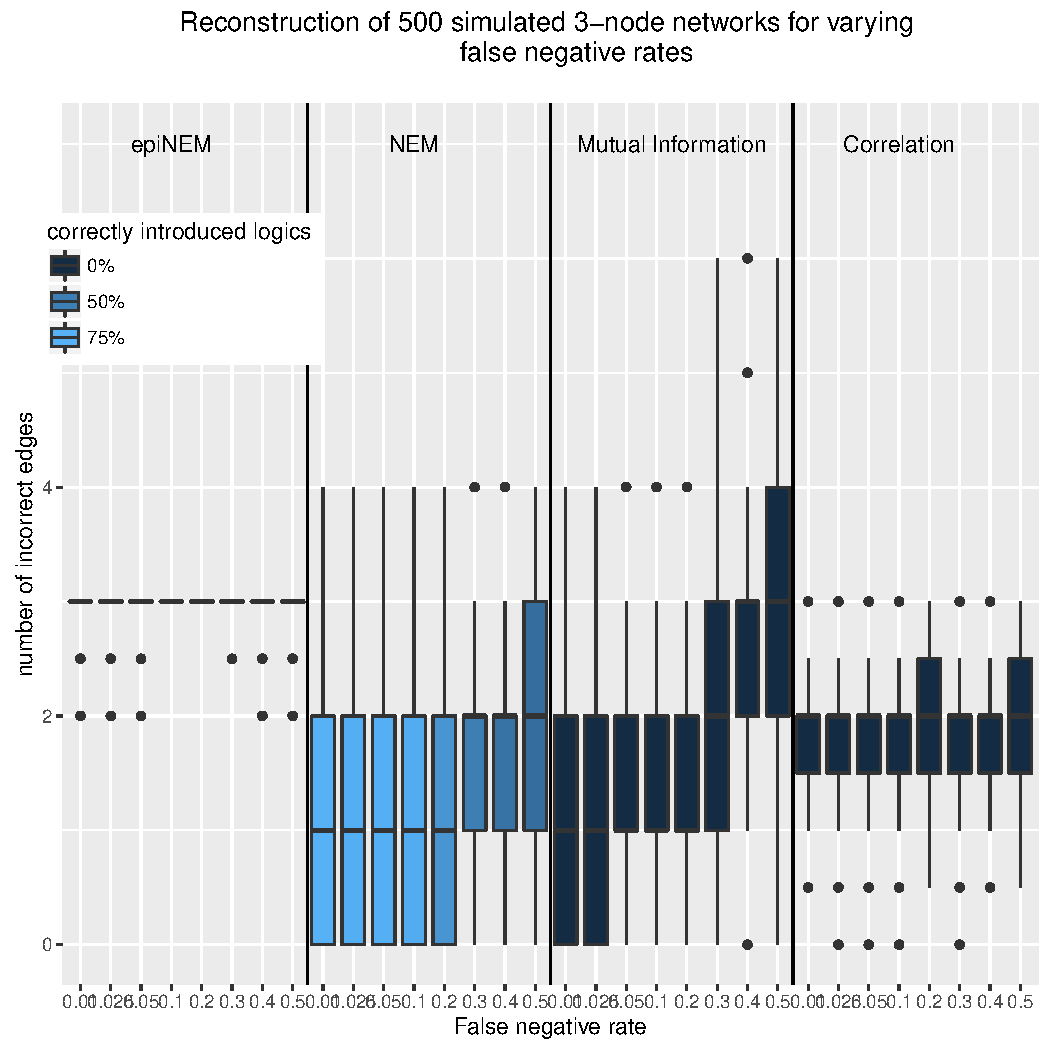
\includegraphics[width=\maxwidth]{figure/unnamed-chunk-4-1} 

\end{knitrout}



\section{Case Study}

\subsection{Data overview}

The data provided in this package is based on the study of van Wageningen [reference]. The dataset consists of in total 150 viable protein kinase and phosphatase perturbations, as well as 15 viable double knockouts. DNA microarray expression profiles were generated under a single growth condition. For each mutant, two independent cultures have been measured and p-values according to relative expression change as well as mutant/wildtype ratios recorded.
The raw data input consists of a matrix of p-values indicating the relative change of gene expression for each perturbation. The columns indicate gene deletions, the rows represent all downstream genes that were investigated for exhibiting effects.

\subsection{Running the main function}

First we load the R packages and load the example data file from \url{http://www.
holstegelab.nl/publications/sv/signaling_redundancy/}. The data file contains a gene expression matrix of all kinase phosphatase mutants. For the analysis, a small number of genes can be selected, which we specify in a 'genelist'.

\begin{knitrout}
\definecolor{shadecolor}{rgb}{0.969, 0.969, 0.969}\color{fgcolor}\begin{kframe}
\begin{alltt}
\hlcom{#library(epiNEM)}
\hlkwd{library}\hlstd{(magrittr)}
\hlkwd{library}\hlstd{(tidyr)}
\hlkwd{library}\hlstd{(ggplot2)}
\hlkwd{library}\hlstd{(data.table)}
\hlkwd{library}\hlstd{(BoolNet)}
\hlkwd{library}\hlstd{(igraph)}
\hlkwd{library}\hlstd{(e1071)}
\hlkwd{library}\hlstd{(grid)}
\hlkwd{library}\hlstd{(org.Sc.sgd.db)}
\hlstd{devtools}\hlopt{::}\hlkwd{load_all}\hlstd{()}
\hlkwd{library}\hlstd{(dplyr)}
\end{alltt}
\end{kframe}
\end{knitrout}

\begin{knitrout}
\definecolor{shadecolor}{rgb}{0.969, 0.969, 0.969}\color{fgcolor}\begin{kframe}
\begin{alltt}
\hlcom{## load data file from local copy or from URL}
\hlstd{address} \hlkwb{<-}
  \hlstr{"http://www.holstegelab.nl/publications/sv/signaling_redundancy/downloads/DataS1.txt"}
\hlstd{data} \hlkwb{<-} \hlkwd{data.table}\hlstd{(}\hlkwd{read.csv}\hlstd{(}\hlkwd{url}\hlstd{(address),} \hlkwc{sep}\hlstd{=}\hlstr{"\textbackslash{}t"}\hlstd{,} \hlkwc{header}\hlstd{=}\hlnum{TRUE}\hlstd{))}
\hlstd{genelist} \hlkwb{<-} \hlkwd{toupper}\hlstd{(}\hlkwd{c}\hlstd{(}\hlstr{'bck1'}\hlstd{,} \hlstr{'slt2'}\hlstd{,} \hlstr{'ptp2'}\hlstd{,} \hlstr{'bck1.slt2'}\hlstd{))}

\hlcom{## read in genes from user and prepare for further analysis}
\hlstd{read_in_genes} \hlkwb{<-} \hlkwa{function}\hlstd{(}\hlkwc{genes}\hlstd{)\{}
  \hlkwd{return}\hlstd{(}\hlkwd{unlist}\hlstd{(}\hlkwd{lapply}\hlstd{(genes,} \hlkwa{function}\hlstd{(}\hlkwc{x}\hlstd{) \{}\hlkwd{paste}\hlstd{(x,} \hlstr{'.del.vs..wt.1'}\hlstd{,} \hlkwc{sep}\hlstd{=}\hlstr{''}\hlstd{)\})))}
\hlstd{\}}
\hlstd{single} \hlkwb{<-} \hlkwd{read_in_genes}\hlstd{(genelist)}
\end{alltt}
\end{kframe}
\end{knitrout}

Also, we only consider changes in expression which result in a p-value < 0.05. All those are set to 1, the other ones to 0.

\begin{knitrout}
\definecolor{shadecolor}{rgb}{0.969, 0.969, 0.969}\color{fgcolor}\begin{kframe}
\begin{alltt}
\hlcom{## numericalize factors}
\hlstd{as.numeric.factor} \hlkwb{<-} \hlkwa{function}\hlstd{(}\hlkwc{x}\hlstd{) \{}\hlkwd{as.numeric}\hlstd{(}\hlkwd{levels}\hlstd{(x))[x]\}}
\end{alltt}
\end{kframe}
\end{knitrout}

Last, we put all constraints together, meaning, we select and binarize the data.

\begin{knitrout}
\definecolor{shadecolor}{rgb}{0.969, 0.969, 0.969}\color{fgcolor}\begin{kframe}
\begin{alltt}
\hlstd{data} \hlopt \hlstd{dplyr}\hlopt{::}\hlkwd{select}\hlstd{(}\hlopt{-}\hlkwd{c}\hlstd{(systematicName, geneSymbol))} \hlopt
  \hlkwd{filter}\hlstd{(}\hlopt{-}\hlnum{1}\hlstd{)} \hlopt
  \hlkwd{mutate_each}\hlstd{(}\hlkwd{funs}\hlstd{(droplevels))} \hlopt
  \hlkwd{mutate_each}\hlstd{(}\hlkwd{funs}\hlstd{(as.numeric.factor))} \hlopt
  \hlkwd{data.frame}\hlstd{()}

\hlcom{# consider foldchange and gene expression}
\hlcom{# 0.73 = log2(1.7)}
\hlstd{new} \hlkwb{<-} \hlkwd{matrix}\hlstd{(}\hlnum{0}\hlstd{,} \hlkwc{ncol}\hlstd{=}\hlkwd{dim}\hlstd{(data)[}\hlnum{2}\hlstd{]}\hlopt{/}\hlnum{2}\hlstd{,} \hlkwc{nrow}\hlstd{=}\hlkwd{dim}\hlstd{(data)[}\hlnum{1}\hlstd{])}
\hlkwd{colnames}\hlstd{(new)} \hlkwb{<-} \hlkwd{colnames}\hlstd{(data)[}\hlnum{1}\hlopt{:}\hlstd{(}\hlkwd{dim}\hlstd{(data)[}\hlnum{2}\hlstd{]}\hlopt{/}\hlnum{2}\hlstd{)]}
\hlstd{n}\hlkwb{=}\hlnum{1}
  \hlkwa{for} \hlstd{(i} \hlkwa{in} \hlkwd{seq}\hlstd{(}\hlnum{1}\hlstd{,} \hlkwd{dim}\hlstd{(data)[}\hlnum{2}\hlstd{],} \hlkwc{by}\hlstd{=}\hlnum{2}\hlstd{))\{}
    \hlkwd{colnames}\hlstd{(new)[n]} \hlkwb{<-} \hlkwd{colnames}\hlstd{(data)[i}\hlopt{+}\hlnum{1}\hlstd{]}
    \hlkwa{for} \hlstd{(k} \hlkwa{in} \hlnum{1}\hlopt{:}\hlkwd{dim}\hlstd{(data)[}\hlnum{1}\hlstd{])\{}
      \hlkwa{if} \hlstd{(((}\hlkwd{abs}\hlstd{(data[k,i]))} \hlopt{>=} \hlnum{0.76}\hlstd{)} \hlopt{&} \hlstd{(data[k,i}\hlopt{+}\hlnum{1}\hlstd{]} \hlopt{<} \hlnum{0.05}\hlstd{))} \hlcom{# & data[k,i+1] > 0))}
        \hlstd{new[k,n]} \hlkwb{<-} \hlnum{1}
      \hlkwa{else} \hlstd{new[k,n]} \hlkwb{<-} \hlnum{0}
    \hlstd{\}}
    \hlstd{n} \hlkwb{=} \hlstd{n}\hlopt{+}\hlnum{1}
  \hlstd{\}}
\hlcom{# filter out 0-rows and set new colnames}
\hlstd{new3} \hlkwb{<-} \hlkwd{data.table}\hlstd{(new[,}\hlkwd{which}\hlstd{(}\hlkwd{colSums}\hlstd{(new)}\hlopt{!=}\hlnum{0}\hlstd{)])}
\hlcom{#new5 <- data.table(new3[which(rowSums(new3)!=0),])}
\hlstd{new4} \hlkwb{<-} \hlstd{new3} \hlopt \hlstd{(}\hlkwa{function}\hlstd{(}\hlkwc{x}\hlstd{)\{}\hlkwd{setnames}\hlstd{(x,} \hlkwd{names}\hlstd{(x),} \hlkwd{toupper}\hlstd{(}\hlkwd{names}\hlstd{(x))} \hlopt
  \hlkwd{gsub}\hlstd{(}\hlstr{'.DEL.VS..WT.1'}\hlstd{,} \hlstr{''}\hlstd{, .)} \hlopt
  \hlkwd{gsub}\hlstd{(}\hlstr{'.VS..WT'}\hlstd{,} \hlstr{''}\hlstd{,.)} \hlopt
  \hlkwd{gsub}\hlstd{(}\hlstr{'.DEL.'}\hlstd{,} \hlstr{'.'}\hlstd{, .));} \hlkwd{return}\hlstd{(x)\})}

\hlstd{mutants}     \hlkwb{<-} \hlkwd{names}\hlstd{(new4)}
\hlstd{experiments} \hlkwb{<-} \hlstd{mutants[}\hlopt{!}\hlkwd{grepl}\hlstd{(}\hlstr{"\textbackslash{}\textbackslash{}."}\hlstd{, mutants)]}
\hlstd{dKO}         \hlkwb{<-} \hlstd{mutants[}\hlkwd{which}\hlstd{(}\hlopt{!}\hlstd{mutants} \hlopt \hlstd{experiments)]}
\hlstd{dKO}         \hlkwb{<-} \hlstd{dKO[}\hlopt{!}\hlkwd{grepl}\hlstd{(}\hlstr{'\textbackslash{}\textbackslash{}..*\textbackslash{}\textbackslash{}.'}\hlstd{, dKO)]}
\hlstd{sKO} \hlkwb{<-} \hlkwd{unlist}\hlstd{(}\hlkwd{strsplit}\hlstd{(dKO,} \hlstr{"."}\hlstd{,} \hlkwc{fixed}\hlstd{=}\hlnum{TRUE}\hlstd{))}

\hlstd{sKO_add} \hlkwb{<-} \hlstd{sKO[}\hlkwd{which}\hlstd{(}\hlopt{!}\hlstd{sKO} \hlopt \hlkwd{names}\hlstd{(new4))]}

\hlkwa{for} \hlstd{(i} \hlkwa{in} \hlnum{1}\hlopt{:}\hlkwd{length}\hlstd{(sKO_add))\{}
  \hlstd{new4[, sKO_add[i]]} \hlkwb{<-} \hlkwd{c}\hlstd{(}\hlkwd{rep}\hlstd{(}\hlnum{0}\hlstd{,}\hlkwd{dim}\hlstd{(new4)[}\hlnum{1}\hlstd{]))}
\hlstd{\}}

\hlstd{PWadd} \hlkwb{<-} \hlstd{genelist[}\hlkwd{which}\hlstd{(}\hlopt{!}\hlstd{genelist} \hlopt \hlkwd{names}\hlstd{(new4))]}
\hlkwa{for}\hlstd{( i} \hlkwa{in} \hlnum{1}\hlopt{:}\hlkwd{length}\hlstd{(PWadd))\{}
  \hlstd{new4[, PWadd[i]]} \hlkwb{<-} \hlkwd{c}\hlstd{(}\hlkwd{rep}\hlstd{(}\hlnum{0}\hlstd{,} \hlkwd{dim}\hlstd{(new4)[}\hlnum{1}\hlstd{]))}
\hlstd{\}}

\hlstd{pathwayData} \hlkwb{<-} \hlstd{new4} \hlopt
  \hlkwd{select_}\hlstd{(}\hlkwc{.dots} \hlstd{= genelist)} \hlopt
  \hlkwd{filter}\hlstd{(}\hlkwd{rowSums}\hlstd{(.)} \hlopt{>} \hlnum{0}\hlstd{)}

\hlcom{# short glimpse of the data}
\hlkwd{head}\hlstd{(pathwayData)}
\end{alltt}
\begin{verbatim}
##    BCK1 SLT2 PTP2 BCK1.SLT2
## 1:    1    0    0         0
## 2:    1    0    0         0
## 3:    0    1    0         0
## 4:    1    0    0         0
## 5:    1    0    0         0
## 6:    1    0    0         0
\end{verbatim}
\end{kframe}
\end{knitrout}

Rownames correspond to sample identifiers. Columns indicate the mutants. A 1 corresponds to a change in expression for an identifier at a knockdown, a 0 represents no effect.

An already processed version of the complete dataset is provided in this package and accessible by calling \emph{epiNEMdata}.

\begin{knitrout}
\definecolor{shadecolor}{rgb}{0.969, 0.969, 0.969}\color{fgcolor}\begin{kframe}
\begin{alltt}
\hlstd{lognem} \hlkwb{<-} \hlkwd{epiNEM}\hlstd{(}\hlkwc{filename}\hlstd{=pathwayData,} \hlkwc{method} \hlstd{=} \hlstr{"exhaustive"}\hlstd{)}\hlcom{#, nIterations=3)}
\end{alltt}
\end{kframe}
\end{knitrout}

epiNEM introduces a logic gate for every node, which has exactly two parents. This logic gate represents the relationship of the parents, the interaction. If there is no interaction, as assumed in the classic NEMs, an OR-gate is introduced. Functional overlap of two genes is represented by an AND-gate, meaning both parents must be knocked out at the same time, in order for the signal to be interrupted. The logics NOTA and NOTB stand for a so called masking effect and the XOR-gate can be interpreted as some kind of mutual prevention of the parents from acting on the child gene.

The search space of epiNEM is now extended by those logic gates, and each model evaluated. Output of the algorithm is all information on the highest-scoring pathway structure.

\begin{knitrout}
\definecolor{shadecolor}{rgb}{0.969, 0.969, 0.969}\color{fgcolor}\begin{kframe}
\begin{alltt}
\hlcom{#lognem <- unlist(lognem, recursive = FALSE)}
\hlstd{lognem}
\end{alltt}
\begin{verbatim}
## [[1]]
## [[1]]$origModel
##      BCK1 PTP2 SLT2
## BCK1    0    1    1
## PTP2    0    0    0
## SLT2    0    1    0
## 
## [[1]]$model
##           BCK1 PTP2 SLT2
## BCK1         1    1    1
## SLT2         0    1    0
## PTP2         0    0    1
## BCK1.SLT2    1    0    1
## 
## [[1]]$logics
##                            Var1 
## "SLT2 masks the effect of BCK1" 
## 
## [[1]]$column
##      c
## [1,] 2
## 
## [[1]]$score
## [1] -41.14147
## 
## [[1]]$EGeneset
##      noE
## BCK1   0
## PTP2   8
## SLT2   0
## null   9
\end{verbatim}
\begin{alltt}
\hlstd{lognem} \hlkwb{<-} \hlkwd{unlist}\hlstd{(lognem,} \hlkwc{recursive} \hlstd{=} \hlnum{FALSE}\hlstd{)}
\end{alltt}
\end{kframe}
\end{knitrout}

\subsection{Plotting the result}

This winning pathway structure can further be visualized by the function PlotResults(), which is also available with the package epiNEM. The grey circles, which are attached to the genes, denote the number of E-genes attached to them. The unconnected circle includes all those, which could not uniquely be attached to a single S-gene.

\begin{knitrout}
\definecolor{shadecolor}{rgb}{0.969, 0.969, 0.969}\color{fgcolor}\begin{kframe}
\begin{alltt}
\hlkwd{epiNEM.PlotResults}\hlstd{(lognem)}
\end{alltt}
\end{kframe}
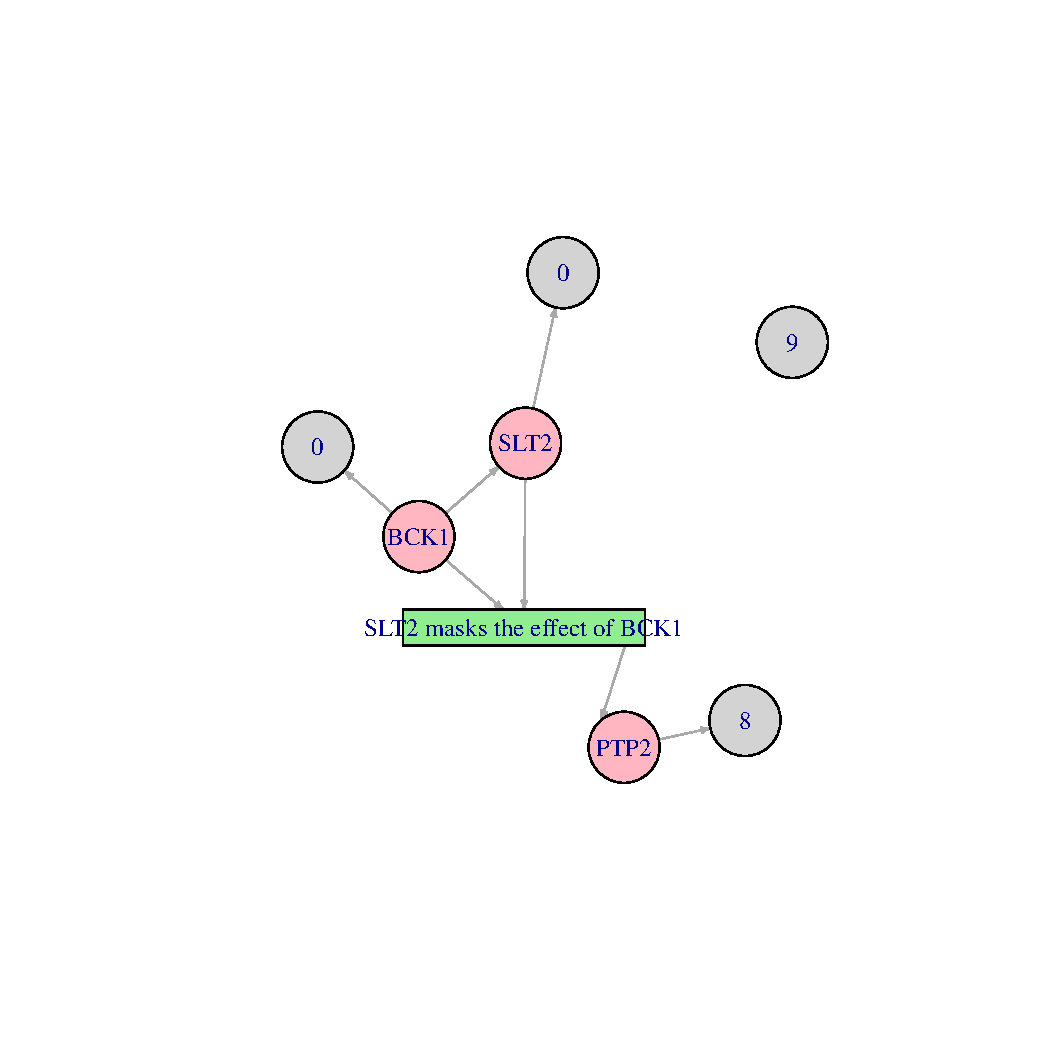
\includegraphics[width=\maxwidth]{figure/unnamed-chunk-11-1} 

\end{knitrout}

\subsection{Triplet screening}

For analysing the mixed epistasis found by van Wageningen et. al., we constructed networks of only three nodes for every double knockout. Or, we combined each pair with any remaining gene and evaluate each of those small networks. Depending on the introduced logic, we were able to confirm most experimental results.
First we need to define the double knockout of interest -- in this example we choose ptp2 and ptp3 -- and combine it with all remaining single experiments in a vector called currentSet.

\begin{knitrout}
\definecolor{shadecolor}{rgb}{0.969, 0.969, 0.969}\color{fgcolor}\begin{kframe}
\begin{alltt}
\hlcom{#  parents     <- 'PTP2.PTP3'}
\hlcom{#  parents2    <- unlist(strsplit(parents, ".", fixed=TRUE))}
\hlcom{#  mutants     <- names(full_matrix)}
\hlcom{#  experiments <- mutants[!grepl("\textbackslash{}\textbackslash{}.", mutants)]}
\hlcom{#  dKO         <- mutants[which(!mutants %in% experiments)]}
\hlcom{#  dKO         <- dKO[!grepl('\textbackslash{}\textbackslash{}..*\textbackslash{}\textbackslash{}.', dKO)]}
\hlcom{#  NOT2 <- paste(parents2[2], "masks the effect of", parents2[1])}
\hlcom{#  NOT1 <- paste(parents2[1], "masks the effect of", parents2[2])}

\hlcom{#  currentSet <- c(experiments, parents)}
\end{alltt}
\end{kframe}
\end{knitrout}
  
  We modify our dataset in a way that it only contains the double knockout of interest plus single knockouts. In addition, we keep a common E-Geneset for better overall comparison of our results. We keep all E-Genes showing effect in either single or double mutant in combination of interest. 

Then, we call epiNEM for every triple in the dataset.

\begin{knitrout}
\definecolor{shadecolor}{rgb}{0.969, 0.969, 0.969}\color{fgcolor}\begin{kframe}
\begin{alltt}
\hlstd{mutants}     \hlkwb{<-} \hlkwd{names}\hlstd{(new4)}
\hlstd{experiments} \hlkwb{<-} \hlstd{mutants[}\hlopt{!}\hlkwd{grepl}\hlstd{(}\hlstr{"\textbackslash{}\textbackslash{}."}\hlstd{, mutants)]}
\hlstd{dKO}         \hlkwb{<-} \hlstd{mutants[}\hlkwd{which}\hlstd{(}\hlopt{!}\hlstd{mutants} \hlopt \hlstd{experiments)]}
\hlstd{dKO}         \hlkwb{<-} \hlstd{dKO[}\hlopt{!}\hlkwd{grepl}\hlstd{(}\hlstr{'\textbackslash{}\textbackslash{}..*\textbackslash{}\textbackslash{}.'}\hlstd{, dKO)]}

\hlcom{#for(tri in 1:length(dKO))\{}
\hlstd{parents}     \hlkwb{<-} \hlstd{dKO[}\hlnum{5}\hlstd{]}
\hlstd{parents2}    \hlkwb{<-} \hlkwd{unlist}\hlstd{(}\hlkwd{strsplit}\hlstd{(parents,} \hlstr{"."}\hlstd{,} \hlkwc{fixed}\hlstd{=}\hlnum{TRUE}\hlstd{))}
\hlstd{NOT2} \hlkwb{<-} \hlkwd{paste}\hlstd{(parents2[}\hlnum{2}\hlstd{],} \hlstr{"masks the effect of"}\hlstd{, parents2[}\hlnum{1}\hlstd{])}
\hlstd{NOT1} \hlkwb{<-} \hlkwd{paste}\hlstd{(parents2[}\hlnum{1}\hlstd{],} \hlstr{"masks the effect of"}\hlstd{, parents2[}\hlnum{2}\hlstd{])}

\hlstd{currentSet} \hlkwb{<-} \hlkwd{c}\hlstd{(experiments, parents)}

\hlstd{trip_data}   \hlkwb{<-} \hlstd{new4} \hlopt \hlcom{#tbl_df() %>%}
    \hlkwd{select_}\hlstd{(.,} \hlkwc{.dots} \hlstd{= currentSet)}

\hlstd{EGcols} \hlkwb{<-} \hlkwd{which}\hlstd{(}\hlkwd{colnames}\hlstd{(trip_data)} \hlopt \hlkwd{c}\hlstd{(parents, parents2))}

\hlstd{trip_data}\hlopt{$}\hlstd{ID} \hlkwb{<-} \hlkwd{as.numeric}\hlstd{(}\hlkwd{rownames}\hlstd{(trip_data))}

\hlcom{## common EGeneset containing only E-genes that are affected at }
\hlcom{## either double or single mutant}
\hlstd{EG} \hlkwb{<-} \hlstd{trip_data} \hlopt
   \hlstd{dplyr}\hlopt{::}\hlkwd{select}\hlstd{(EGcols, ID)} \hlopt
   \hlkwd{filter}\hlstd{((}\hlkwd{rowSums}\hlstd{(.)}\hlopt{-}\hlstd{ID)} \hlopt{>} \hlnum{0}\hlstd{)}

\hlstd{EGdata} \hlkwb{<-} \hlkwd{as.data.frame}\hlstd{(trip_data)[}\hlkwd{which}\hlstd{(trip_data}\hlopt{$}\hlstd{ID} \hlopt \hlstd{EG}\hlopt{$}\hlstd{ID),]}

  \hlstd{scores} \hlkwb{<-} \hlkwd{c}\hlstd{()}
  \hlstd{singles} \hlkwb{<-} \hlstd{experiments[}\hlkwd{which}\hlstd{(}\hlopt{!}\hlstd{experiments} \hlopt \hlstd{parents2)]}
\hlkwa{for} \hlstd{(i} \hlkwa{in} \hlnum{1}\hlopt{:}\hlstd{(}\hlkwd{length}\hlstd{(singles)}\hlopt{-}\hlnum{1}\hlstd{))\{}
  \hlstd{mutants1}    \hlkwb{<-} \hlkwd{c}\hlstd{(singles[i], parents2, parents)}
  \hlstd{experiments1} \hlkwb{<-} \hlstd{mutants1[}\hlnum{1}\hlopt{:}\hlkwd{length}\hlstd{(mutants1)}\hlopt{-}\hlnum{1}\hlstd{]}
  \hlstd{modelsTrip1} \hlkwb{<-} \hlkwd{EnumerateModels}\hlstd{(}\hlkwd{length}\hlstd{(experiments1), experiments1)}
  \hlstd{EGdata2}     \hlkwb{<-} \hlstd{EGdata[,}\hlkwd{which}\hlstd{(}\hlkwd{colnames}\hlstd{(trip_data)} \hlopt \hlstd{mutants1)]}
  \hlstd{scores[[i]]} \hlkwb{<-} \hlkwd{epiNEM}\hlstd{(}\hlkwc{filename} \hlstd{= EGdata2,} \hlkwc{method} \hlstd{=} \hlstr{"exhaustive"}\hlstd{)}
  \hlcom{#load('SAgain_scores6_12.RData')}
\hlstd{\}}
\end{alltt}
\end{kframe}
\end{knitrout}



And finally we can plot the marginal likelihood and the logic included for evaluation. In this example it shows clearly, that only AND-logic gates were introduced to every single model. This overlaps with the results from van Wageningen et. al. who found out experimentally, that ptp2 with ptp3 always behave in complete redundancy.

\begin{knitrout}
\definecolor{shadecolor}{rgb}{0.969, 0.969, 0.969}\color{fgcolor}
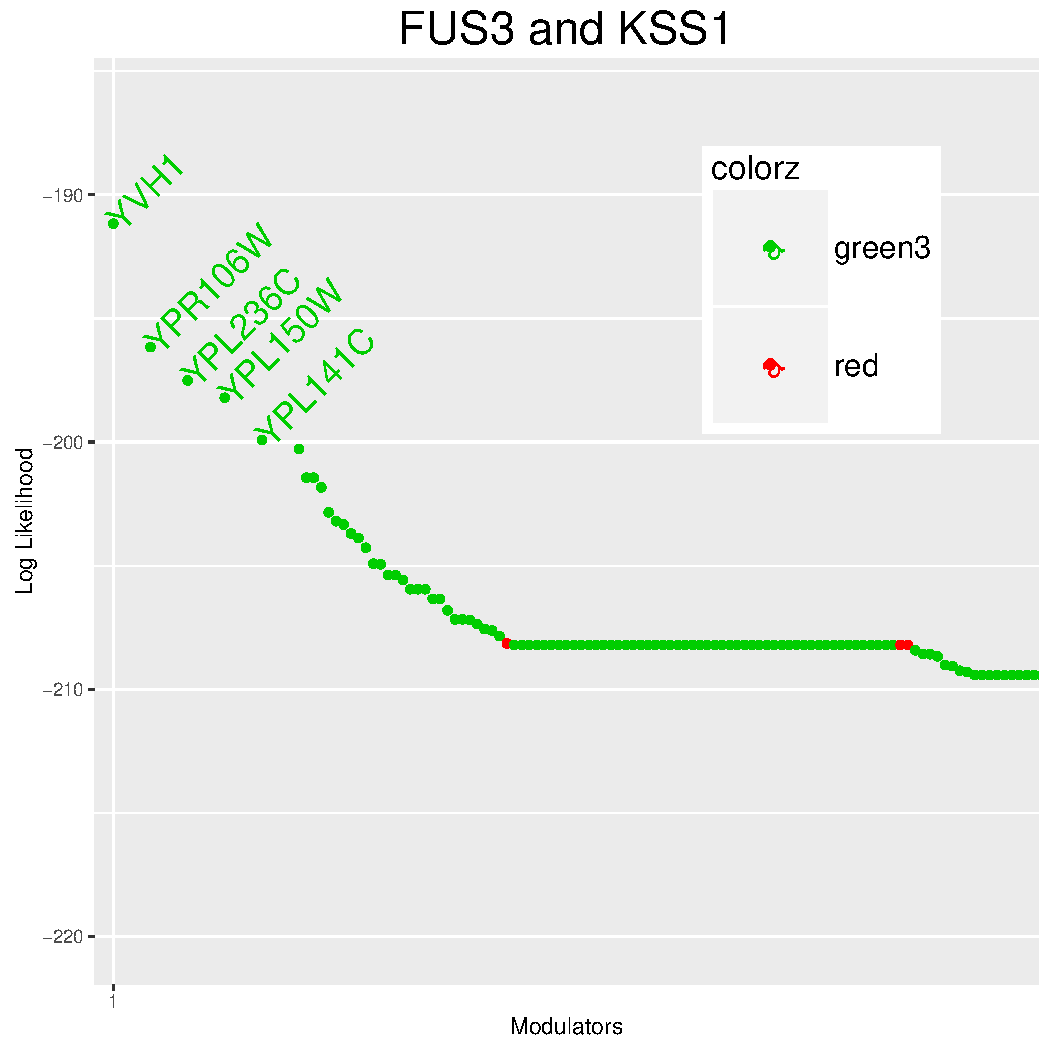
\includegraphics[width=\maxwidth]{figure/unnamed-chunk-15-1} 

\end{knitrout}
%%%%%%%%%%%%%%%%%%%%%%%%%%%%%%%%%%%%%%%%%%%%%%%%%%%%

        
%%
%%
%%%%%%%%%%%%%%%%%%%%%%%%%%%%%%%%%%%%%%%%%%%%%%%%%%%%
\clearpage
\section{Session Info}
\begin{knitrout}
\definecolor{shadecolor}{rgb}{0.969, 0.969, 0.969}\color{fgcolor}\begin{kframe}
\begin{alltt}
\hlkwd{sessionInfo}\hlstd{()}
\end{alltt}
\begin{verbatim}
## R version 3.2.1 (2015-06-18)
## Platform: x86_64-apple-darwin13.4.0 (64-bit)
## Running under: OS X 10.10.4 (Yosemite)
## 
## locale:
## [1] C
## 
## attached base packages:
##  [1] parallel  stats4    grid      stats     graphics  grDevices utils    
##  [8] datasets  methods   base     
## 
## other attached packages:
##  [1] epiNEM_0.0.0.9000    dplyr_0.4.3          org.Sc.sgd.db_3.2.3 
##  [4] RSQLite_1.0.0        DBI_0.3.1            AnnotationDbi_1.32.3
##  [7] IRanges_2.4.6        S4Vectors_0.8.7      Biobase_2.30.0      
## [10] BiocGenerics_0.16.1  e1071_1.6-7          igraph_1.0.1        
## [13] BoolNet_2.1.1        data.table_1.9.6     ggplot2_2.0.0       
## [16] tidyr_0.4.0          magrittr_1.5         knitr_1.12          
## 
## loaded via a namespace (and not attached):
##  [1] Rcpp_0.12.3      formatR_1.2.1    plyr_1.8.3       highr_0.5.1     
##  [5] class_7.3-14     tools_3.2.1      digest_0.6.9     evaluate_0.8    
##  [9] memoise_0.2.1    gtable_0.1.2     stringr_1.0.0    roxygen2_5.0.1  
## [13] devtools_1.9.1   R6_2.1.1         XML_3.98-1.3     scales_0.3.0    
## [17] assertthat_0.1   colorspace_1.2-6 labeling_0.3     stringi_1.0-1   
## [21] lazyeval_0.1.10  munsell_0.4.2    chron_2.3-47
\end{verbatim}
\end{kframe}
\end{knitrout}

%%%%%%%%%%%%%%%%%%%%%%%%%%%%%%%%%%%%%%%%%%%%%%%%%%%%%%%%%%%%%%%%%%%%%%
%% References
%%%%%%%%%%%%%%%%%%%%%%%%%%%%%%%%%%%%%%%%%%%%%%%%%%%%%%%%%%%%%%%%%%%%%%
%\clearpage
\bibliographystyle{../manuscript/myvancouver}
\bibliography{../manuscript/cnv-distance}



\end{document}

